\chapter{Graph Algorithms}

\begin{definitionblock}[Graph]
A graph $G$ is a pair $(V, E)$, where $V$ is a set of vertices and $E$ is a set of edges. Each edge is a pair of vertices.
\end{definitionblock}

We can choose between two standard ways to represent a graph $G = (V,E)$:
as a collection of adjacency lists or as an adjacency matrix. Either way applies
to both directed and undirected graphs. Because the adjacency-list representation
provides a compact way to represent sparse graphs, it is usually the method of choice.

\begin{figure}[H]
    \centering
    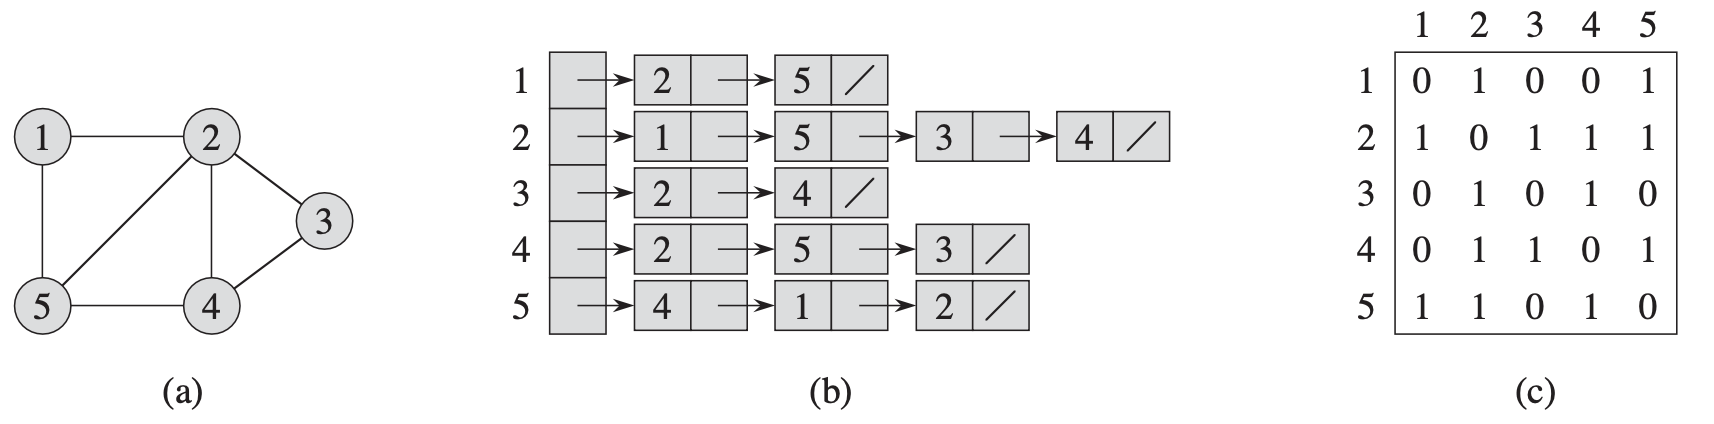
\includegraphics[width=0.9\textwidth]{assets/undirected_graph.png}
    \caption{Undirected raph}
    \label{fig:undirected_graph}

    \vspace{1em}

    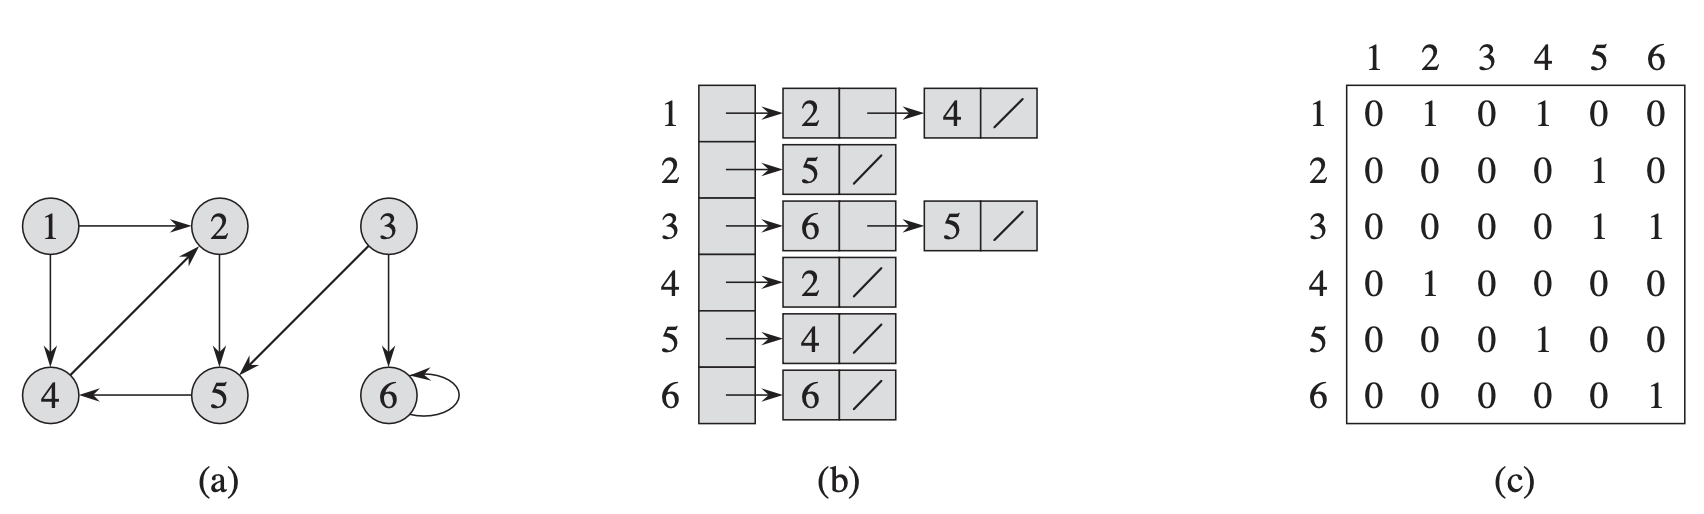
\includegraphics[width=0.9\textwidth]{assets/directed_graph.png}
    \caption{Directed graph}
    \label{fig:directed_graph}
\end{figure}

\begin{itemize}
    \item \textbf{Path}: A path in a graph is a sequence of vertices $v_1, v_2, \ldots, v_n$ such that $(v_i, v_{i+1}) \in E$ for $1 \leq i \leq n - 1$. The length of the path is the number of edges in the path, which is $n - 1$.
    \item \textbf{Walk}: A walk in a graph is a sequence of vertices $v_1, v_2, \ldots, v_n$ such that $(v_i, v_{i+1}) \in E$ for $1 \leq i \leq n - 1$. The length of the walk is the number of edges in the walk, which is $n - 1$.
    \item \textbf{Cycle}: A cycle in a graph is a path of length at least 1, whose first and last vertices are the same.
    \item \textbf{Connected component}: A connected component of an undirected graph $G = (V, E)$ is a maximal set of vertices $C \subseteq V$ such that for every pair of vertices $u, v \in C$, there is a path from $u$ to $v$.
\end{itemize}

\subsection*{Graph Representation}

The \textbf{adjacency-list representation} of a graph $G = (V, E)$ consists of an array $Adj$ of $|V|$ lists, one for each vertex in $V$. For each vertex $u \in V$, the adjacency list $Adj[u]$ contains all the vertices $v$ such that there is an edge $(u, v) \in E$. That is, $Adj[u]$ is a list of all the vertices adjacent to $u$ in $G$.
We can adapt the adjacency-list representation to represent weighted graphs by storing, for each vertex $v$, not only the vertices adjacent to $v$ but also the weights of the edges incident on $v$.

The \textbf{adjacency-matrix representation} of a graph $G = (V, E)$ consists of a $|V| \times |V|$ matrix $W = (w_{ij})$, where
$$
    w_{ij} = 
    \begin{cases}
        1 & \text{if } (i, j) \in E, \\
        0 & \text{otherwise}.
    \end{cases}
$$
The adjacency-matrix representation is particularly convenient when the graph is dense, that is, when $|E|$ is close to $|V|^2$.

\section{Breadth-First Search}

Given a graph $G = (V, E)$ and a distinguished source vertex $s$, breadth-first search systematically explores the edges of $G$ to discover every vertex that is reachable from $s$. It computes the distance (smallest number of edges) from $s$ to each reachable vertex.
It also produces a \textbf{breadth-first tree} with root $s$ that contains all reachable vertices. For any vertex $v$ reachable from $s$, the simple path in the breadth-first tree from $s$ to $v$ corresponds to a shortest path from $s$ to $v$ in $G$, that is, a path containing the smallest number of edges.
The algorithm discovers all vertices at distance $k$ from $s$ before discovering any
vertices at distance $k+1$.

\begin{observationblock}[Data structure used]
The algorithm uses a first-in first-out queue $Q$ to manage the set of gray vertices. 
\end{observationblock}

\begin{figure}[H]
    \centering
    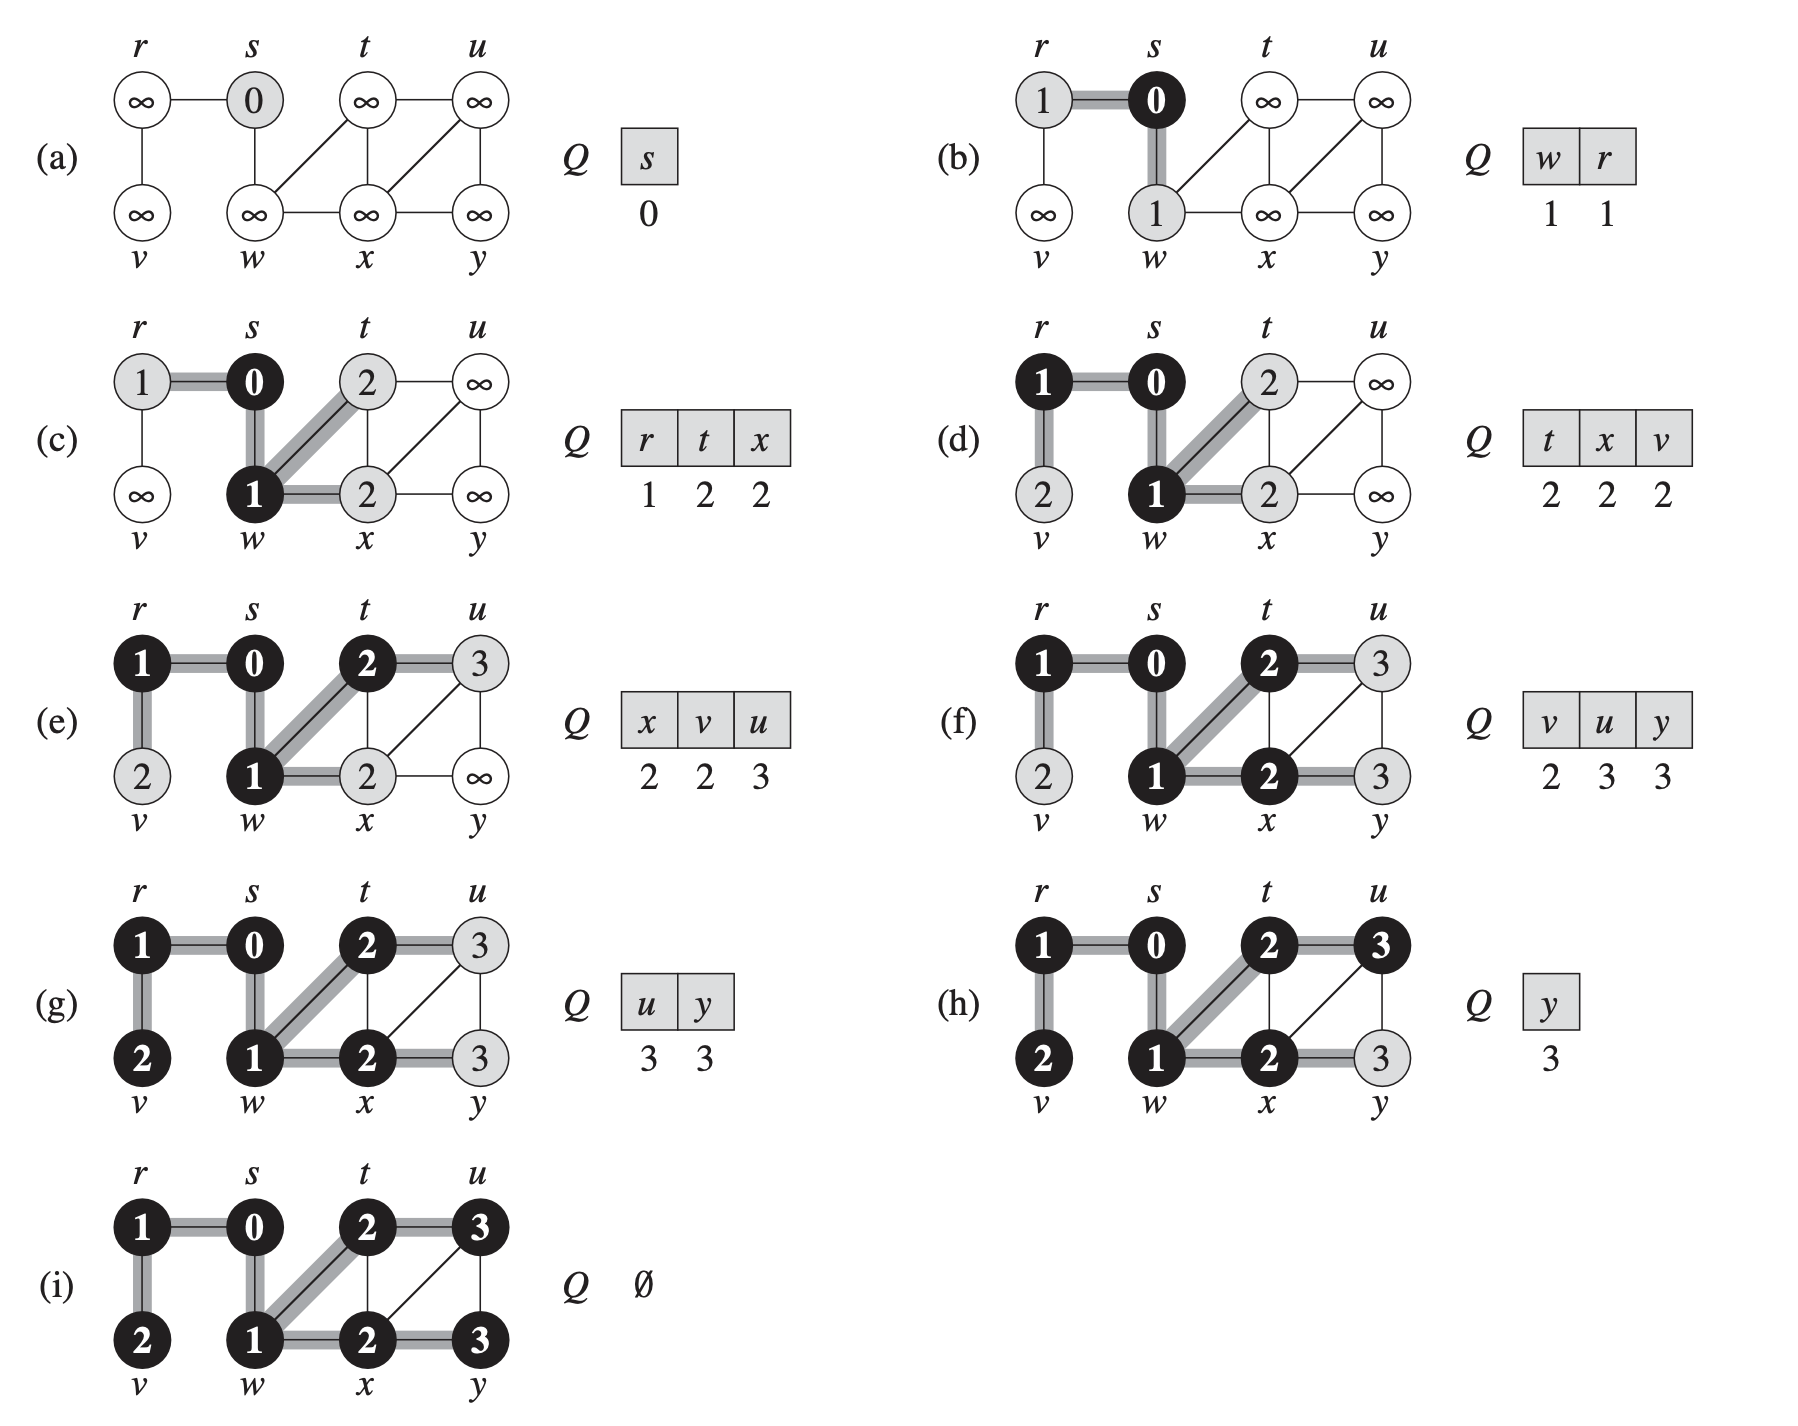
\includegraphics[width=0.6\textwidth]{assets/bfs.png}
    \caption{Breadth-First Search}
    \label{fig:bfs}
\end{figure}

\begin{algorithm}[H]
    \caption{BFS(G, s)}
    \begin{algorithmic}[1]
        \For{each vertex u $\in$ V - \{s\}} \Comment{Initialization: $O(|V|)$}
            \State color[u] $\gets$ WHITE
            \State d[u] $\gets \infty$
            \State $\pi$[u] $\gets$ NIL
        \EndFor
        \State 
        \State color[s] $\gets$ GRAY \Comment{Visit of the source: $O(1)$}
        \State d[s] $\gets$ 0
        \State $\pi$[s] $\gets$ NIL
        \State Q $\gets \emptyset$
        \State ENQUEUE(Q, s)
        \State 
        \While{Q $\neq \emptyset$} \Comment{Visit of the vertices: $O(|E|)$}
            \State u $\gets$ DEQUEUE(Q)
            \For{each vertex $v$ $\in$ Adj[u]}
                \If{color[v] = WHITE}
                    \State color[v] $\gets$ GRAY
                    \State d[v] $\gets$ d[u] + 1
                    \State $\pi$[v] $\gets$ u
                    \State ENQUEUE(Q, v)
                \EndIf
            \EndFor
            \State color[u] $\gets$ BLACK
        \EndWhile
    \end{algorithmic}
\end{algorithm}

\subsection*{Analysis}

After initialization, breadth-first search never whitens a vertex, and thus the test in line 13 ensures that each vertex is enqueued at most once, and hence dequeued at most once. The operations of enqueuing and dequeuing take $O(1)$ time, and so the total time devoted to queue operations is $O(V)$. Because the procedure scans the adjacency list of each vertex only when the vertex is dequeued, it scans each adjacency list at most once. Since the sum of the lengths of all the adjacency lists is $\Theta(E)$, the total time spent in scanning adjacency lists is $O(E)$. The overhead for initialization is $O(V)$, and thus the total running time of the BFS procedure is $O(V + E)$. Thus, breadth-first search runs in time linear in the size of the adjacency-list representation of $G$.

\newpage

\subsection*{Shortest Paths}

\begin{definitionblock}[Shortest Path Distance]
    Define the \textbf{shortest path distance} $\delta(s,v)$ from $s$ to $v$ as the minimum number of edges in any path from vertex $s$ to vertex $v$; if there is no path from $s$ to $v$, then $\delta(s,v) = \infty$.
\end{definitionblock}

\newtheorem{shortest path}{Lemma}
\begin{theorem}
    Let $G = (V, E)$ be a directed or undirected graph, and let $s \in V$ be an arbitrary
    vertex. Then, for any edge $(u, v) \in E$, $\delta(s, v) \leq \delta(s, u) + 1$.
\end{theorem}

\begin{proof}
    If $u$ is reachable from $s$, then so is $v$. In this case, the shortest path from $s$
    to $v$ cannot be longer than the shortest path from $s$ to $u$ followed by the edge $(u,v)$,
    and thus the inequality holds. If $u$ is not reachable from $s$, then $\delta(s,v) = \infty$, and
    the inequality holds.
\end{proof}

\newtheorem{shortest path 2}{Lemma}
\begin{theorem}
    Let $G = (V, E)$ be a directed or undirected graph, and suppose BFS is run on G
    from a given source $s \in V$. Then upon termination, for each vertex $v \in V$, 
    the value $v.d$ computed by the BFS satisfies $v.d \geq \delta(s, v)$.
\end{theorem}
\begin{proof}
    We prove this theorem by induction on the number of vertices in the breadth-first tree.

    \textbf{Base case:} The base case is the source vertex $s$. Initially, $s.d = 0$ and $\delta(s, s) = 0$. Therefore, $s.d = \delta(s, s)$, and the base case holds.

    \textbf{Inductive step:} Assume that for any vertex $u$ in the breadth-first tree, $u.d \geq \delta(s, u)$. We need to show that for any vertex $v$ adjacent to $u$, $v.d \geq \delta(s, v)$.

    When $v$ is first discovered, it is enqueued and $v.d$ is set to $u.d + 1$. By the inductive hypothesis, $u.d \geq \delta(s, u)$. Therefore, $v.d = u.d + 1 \geq \delta(s, u) + 1$. Since $(u, v)$ is an edge in the graph, $\delta(s, v) \leq \delta(s, u) + 1$. Combining these inequalities, we get $v.d \geq \delta(s, u) + 1 \geq \delta(s, v)$.

    Thus, by induction, for each vertex $v \in V$, the value $v.d$ computed by BFS satisfies $v.d \geq \delta(s, v)$.
\end{proof}

\newtheorem{correctedness of bfs}{Lemma}
\begin{theorem}
    Let $G = (V, E)$ be a directed or undirected graph and suppose BFS is run on G 
    from a given source $s \in V$. Then during its execution, BFS discovers every vertex
    $v \in V$ that is reachable from $s$, and upon termination, $v.d = \delta(s, v)$.
    Moreover, for any vertex $v \neq s$ that is reachable from s, one of the shortest paths 
    from $s$ to $v$ is a shortest path from $s$ to $v.\pi$ followed by the edge $(v.\pi, v)$.
\end{theorem}
\begin{proof}
    Assume, for the purpose of contradiction, that some vertex $v$ receives a $d$-value not equal to its shortest-path distance $\delta(s, v)$. Let $v$ be the vertex with the minimum $\delta(s, v)$ that receives such an incorrect $d$-value. Clearly, $v \neq s$. Since 
    $v.d \geq \delta(s, v)$, 
    we have 
    $v.d > \delta(s, v)$. 
    Vertex $v$ must be reachable from $s$; otherwise, 
    $\delta(s, v) = \infty > v.d$. 
    Let $u$ be the vertex immediately preceding $v$ on a shortest path from $s$ to $v$, so that 
    $\delta(s, v) = \delta(s, u) + 1$. 
    Because 
    $v.d > \delta(s, v)$, 
    it follows that 
    $v.d = \delta(s, u) + 1 = u.d + 1$. 

    Now consider when BFS dequeues $u$ from $Q$. At this time, $v$ can be white, gray, or black:
    \begin{itemize}
        \item If $v$ is white, line 15 sets 
        $v.d = u.d + 1$, 
        contradicting 
        $v.d > \delta(s, v)$.

        \item If $v$ is black, $v$ has already been removed from the queue, so 
        $v.d \leq u.d$, 
        again contradicting 
        $v.d > \delta(s, v)$.

        \item If $v$ is gray, it was painted gray during the dequeue of some vertex $w$, removed from $Q$ earlier than $u$. Since 
        $w.d \leq u.d$, 
        it follows that 
        $v.d = w.d + 1 \leq u.d + 1$, 
        again contradicting 
        $v.d > \delta(s, v)$.
    \end{itemize}

    Thus, $v.d = \delta(s, v)$ for all $v \in V$. Since all vertices reachable from $s$ must be discovered, the proof is complete. Finally, if $v.\pi = u$, then $v.d = u.d + 1$, ensuring that a shortest path from $s$ to $v$ is obtained by traversing $(v.\pi, v)$.
\end{proof}

\newpage

\section{Single Source Shortest Paths}

In a \textbf{shortest-path problem}, we are given a weighted, directed graph $G = (V, E)$, with weight function $w : E \to \mathbb{R}$ mapping edges to 
real-values weights. the \textbf{weight} $w(p)$ of path $p = \langle v_0,v_1,\dots,v_k \rangle$ is the sum of the weights of its constituent edges:

$$
    w(p) = \sum_{i=1}^{k} w(v_{i-1}, v_i)
$$

We define the \textbf{shortest-path weight} $\delta(u,v)$ from $u$ to $v$ as the minimum weight of any path from $u$ to $v$:

$$
    \delta(u,v) = 
    \begin{cases}
        \min \{ w(p) : \text{p is a path from u to v} \} & \text{if there is a path from u to v}, \\
        \infty & \text{otherwise}.
    \end{cases}
$$

\begin{warningblock}[BFS]
BFS is used to compute shortest paths in unweighted graphs. In weighted graphs, BFS can be used to compute shortest paths only when all edge weights are equal.
\end{warningblock}

\newtheorem{subpaths}{Lemma}
\begin{theorem}
    Given a weighted, directed graph $G = (V, E)$ with weight function $w : E \to \mathbb{R}$, let $p = \langle v_0, v_1, \dots, v_k \rangle$ be a shortest path from vertex $v_0$ to vertex $v_k$. For any $i$ and $j$ such that $0 \leq i \leq j \leq k$, let $p_{ij} = \langle v_i, v_{i+1}, \dots, v_j \rangle$ be the subpath of $p$ from vertex $v_i$ to vertex $v_j$. Then, $p_{ij}$ is a shortest path from $v_i$ to $v_j$.
\end{theorem}
\begin{proof}
    Decompose the path $p$ into three segments: $p_{0i}$ from $v_0$ to $v_i$, $p_{ij}$ from $v_i$ to $v_j$, and $p_{jk}$ from $v_j$ to $v_k$. Then, the weight of $p$ is given by:
    $$
    w(p) = w(p_{0i}) + w(p_{ij}) + w(p_{jk}).
    $$
    Assume there exists a path $p'_{ij}$ from $v_i$ to $v_j$ with weight $w(p'_{ij}) < w(p_{ij})$. Then, the path $p' = \langle p_{0i}, p'_{ij}, p_{jk} \rangle$ would have weight:
    $$
    w(p') = w(p_{0i}) + w(p'_{ij}) + w(p_{jk}),
    $$
    which is less than $w(p)$. This contradicts the assumption that $p$ is a shortest path from $v_0$ to $v_k$. Thus, $p_{ij}$ must be a shortest path from $v_i$ to $v_j$. 
\end{proof}

\subsection*{Cycles}

\begin{itemize}
    \item \textbf{Positive cycle}: A cycle whose edges have a positive sum of weights.
    \item \textbf{Negative cycle}: A cycle whose edges have a negative sum of weights. It makes the cost of a path not well defined cause each cycle creates lower cost each time. 
\end{itemize}

A shortest path cannot contain a negative cycle. If a negative cycle is reachable from the source vertex, then there is no shortest path, since the path can be made as short as desired by traversing the negative cycle arbitrarily many times.
Nor it can contain a positive cycle, since the path can be made shorter by removing the cycle.

\begin{figure}[H]
    \centering
    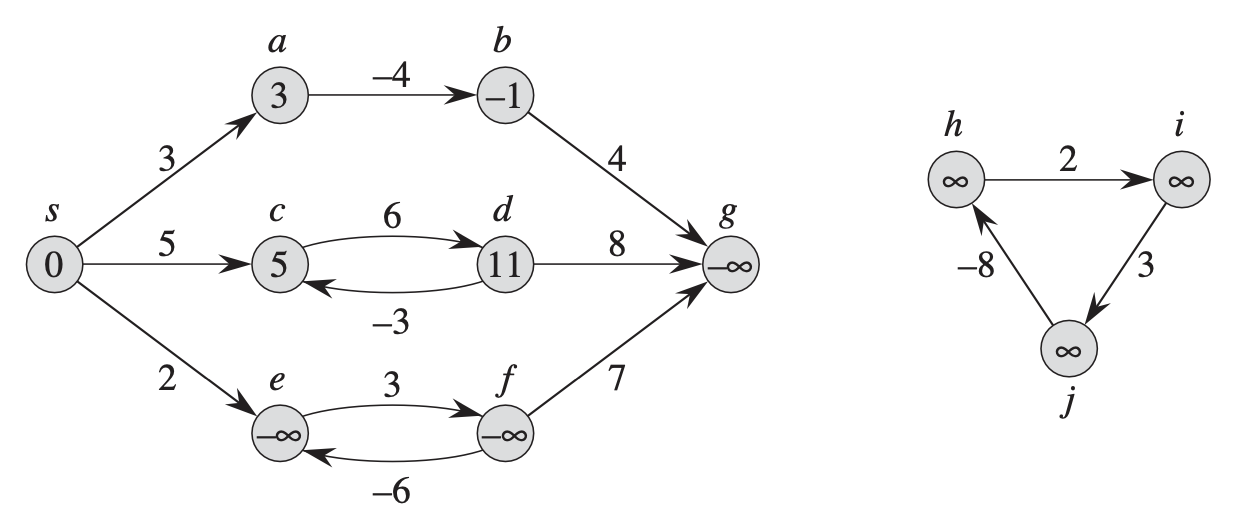
\includegraphics[width=0.8\textwidth]{assets/neg_cycle.png}
    \caption{Negative cycle}
    \label{fig:negative_cycle}
\end{figure}

\subsection*{Representation}

To compute shortest paths, not only the weights but also the vertices on the paths are maintained. For a graph $G = (V, E)$, each vertex $v \in V$ has a predecessor $\pi(v)$, which is either another vertex or $\text{NIL}$. The $\pi$ values represent the chain of predecessors that define the shortest path from a source vertex $s$ to $v$. The procedure \texttt{PRINT-PATH}$(G, s, v)$ can reconstruct this shortest path.

In shortest-path algorithms, the $\pi$ values define a \textit{predecessor subgraph} $G_\pi = (V_\pi, E_\pi)$:

$$
V_\pi = \{v \in V : \pi(v) \neq \text{NIL}\} \cup \{s\},
\\
E_\pi = \{(\pi(v), v) \in E : v \in V_\pi \setminus \{s\}\}.
$$

At termination, $G_\pi$ forms a \textit{shortest-path tree}, which is a rooted tree with:

\begin{enumerate}
    \item $V'$, the set of vertices reachable from $s$ in $G$.
    \item A root at $s$ and edges $E'$ such that:
    \begin{itemize}
        \item $V' \subseteq V$,
        \item $E' \subseteq E$.
    \end{itemize}
    \item For all $v \in V'$, the unique simple path from $s$ to $v$ in $G'$ is the shortest path in $G$.
\end{enumerate}

A shortest-path tree extends the concept of a breadth-first tree to account for edge weights.

\begin{figure}[H]
    \centering
    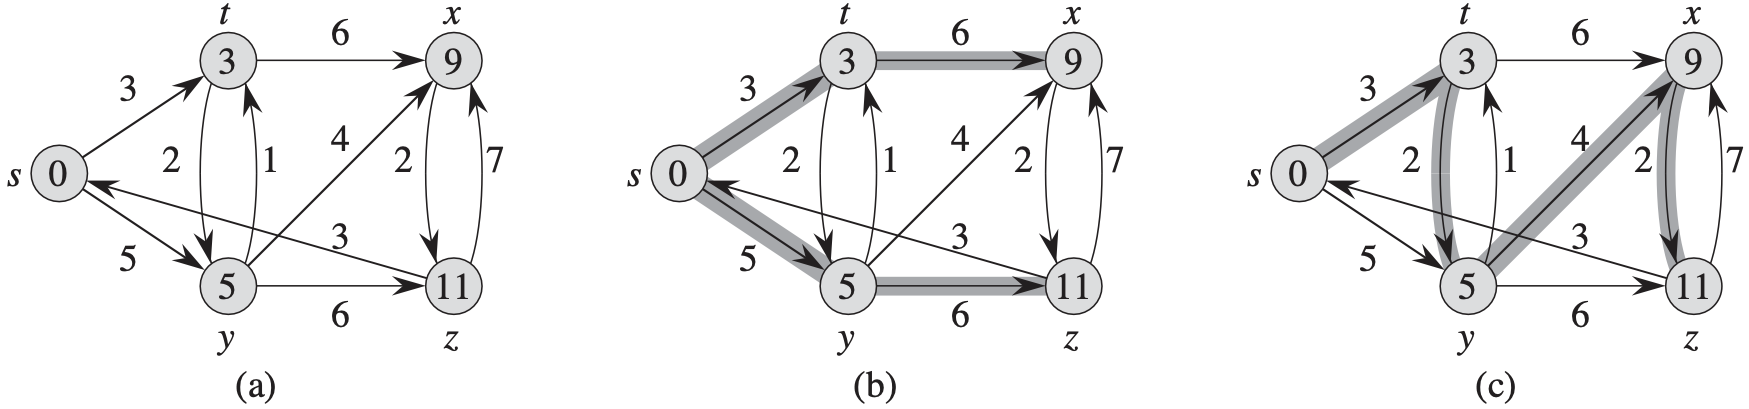
\includegraphics[width=\textwidth]{assets/representation_shortest_path.png}
    \caption{Shortest-path representation}
    \label{fig:representation_shortest_path}
\end{figure}

\subsection*{Relaxation}

For each vertex $v \in V$, we maintain an attribute $v.d$ that is an upper bound on the weight of a shortest path from source $s$ to $v$. We call $v.d$ a \textbf{shortest-path estimate}. We initialize the shortest-path estimates and predecessors by the following $\Theta(V)$-time procedure:

\begin{algorithm}[H]
    \caption{INITIALIZE-SINGLE-SOURCE(G, s)}
    \begin{algorithmic}[1]
        \For{each vertex $v$ $\in$ V}
            \State v.d $\gets \infty$
            \State $\pi$(v) $\gets$ NIL
        \EndFor
        \State s.d $\gets$ 0
    \end{algorithmic}
\end{algorithm}

\vspace{-1em}

The process of \textbf{relaxing} an edge $(u, v)$ consists of testing whether we can improve the shortest path to found so far by going through u and, if so, updating $v.d$ and $v.\pi$.
A relaxation step may decrease the value of $v.d$ and update $v.\pi$. The following code performs a relaxation step on edge $(u, v)$:

\begin{algorithm}[H]
    \caption{RELAX(u, v, w)}
    \begin{algorithmic}[1]
        \If{v.d > u.d + w(u, v)}
            \State v.d $\gets$ u.d + w(u, v)
            \State v.$\pi$ $\gets$ u
        \EndIf
    \end{algorithmic}
\end{algorithm}

\vspace{-1em}

\begin{figure}[H]
    \centering
    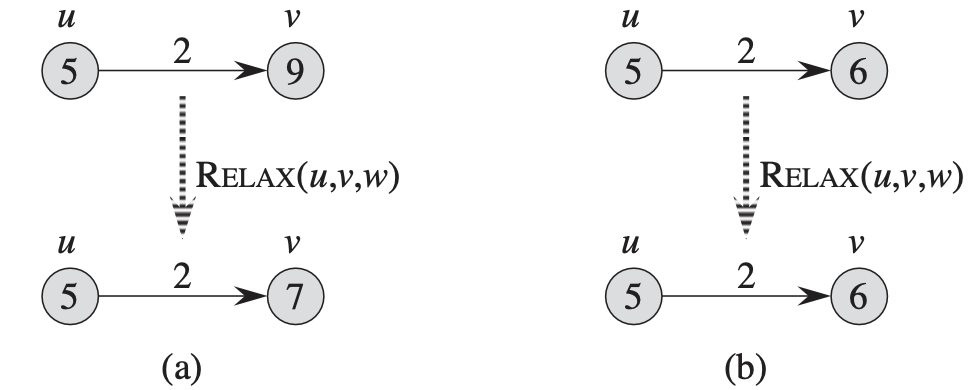
\includegraphics[width=0.6\textwidth]{assets/relaxation.png}
    \caption{Relaxation}
    \label{fig:relaxation}
\end{figure}

\vspace{-1em}

\subsection*{Bellman-Ford Algorithm}

\vspace{-1em}

\begin{algorithm}[H]
    \caption{Bellman-Ford(G, w, s)}
    \begin{algorithmic}[1]
        \State INITIALIZE-SINGLE-SOURCE(G, s)
        \For{i = 1 \textbf{ to } |V| - 1}
            \For{each edge (u, v) $\in$ E}
                \State RELAX(u, v, w)
            \EndFor
        \EndFor
        \For{each edge (u, v) $\in$ E}
            \If{v.d > u.d + w(u, v)}
                \State \Return FALSE
            \EndIf
        \EndFor
        \State \Return TRUE
    \end{algorithmic}
\end{algorithm}

\vspace{-1em}

\begin{warningblock}[Bellman-Ford]
This algorithm can be used to detect negative cycles. If the algorithm returns \plaintt{FALSE}, then there is a negative cycle reachable from the source vertex.
This means that it \textbf{does not} work with negaive cycles.
\end{warningblock}

\newpage

\section{Depth-First Search}

The strategy followed by depth-first search is, as its name implies, to search “deeper” in the graph whenever possible. Depth-first search explores edges out of the most recently discovered vertex that still has unexplored edges leaving it. Once all of ’s edges have been explored, the search “backtracks” to explore edges leaving the vertex from which was discovered. This process continues until we have discovered all the vertices that are reachable from the original source vertex. If any undiscovered vertices remain, then depth-first search selects one of them as a new source, and it repeats the search from that source. The algorithm repeats this entire process until it has discovered every vertex.

Unlike breadth-first search,whose predecessor subgraph forms a tree, the predecessor subgraph produced by a depth-first search may be composed of several trees, because the search may repeat from multiple sources. Therefore, we define the predecessor subgraph of a depth-first search slightly differently from that of a breadth-first search: we let $G_{\pi} = (V, E_{\pi})$, where $E_{\pi} = \{(\pi(v), v) : v \in V \text{ and } \pi(v) \neq \text{NIL}\}$.

The predecessor subgraph of a depth-first search forms a depth-first forest comprising several depth-first trees.

As in breadth-first search, depth-first search colors vertices during the search to indicate their state. Each vertex is initially white, is grayed when it is discovered in the search, and is blackened when it is finished, that is, when its adjacency list has been examined completely.

Besides creating a depth-first forest, depth-first search also assigns each vertex $v$ two timestamps: a discovery time $v.d$ when $v$ is first visited (colored gray), and a finishing time $v.f$ when $v$'s adjacency list is fully examined (colored black).

\begin{figure}[H]
    \centering
    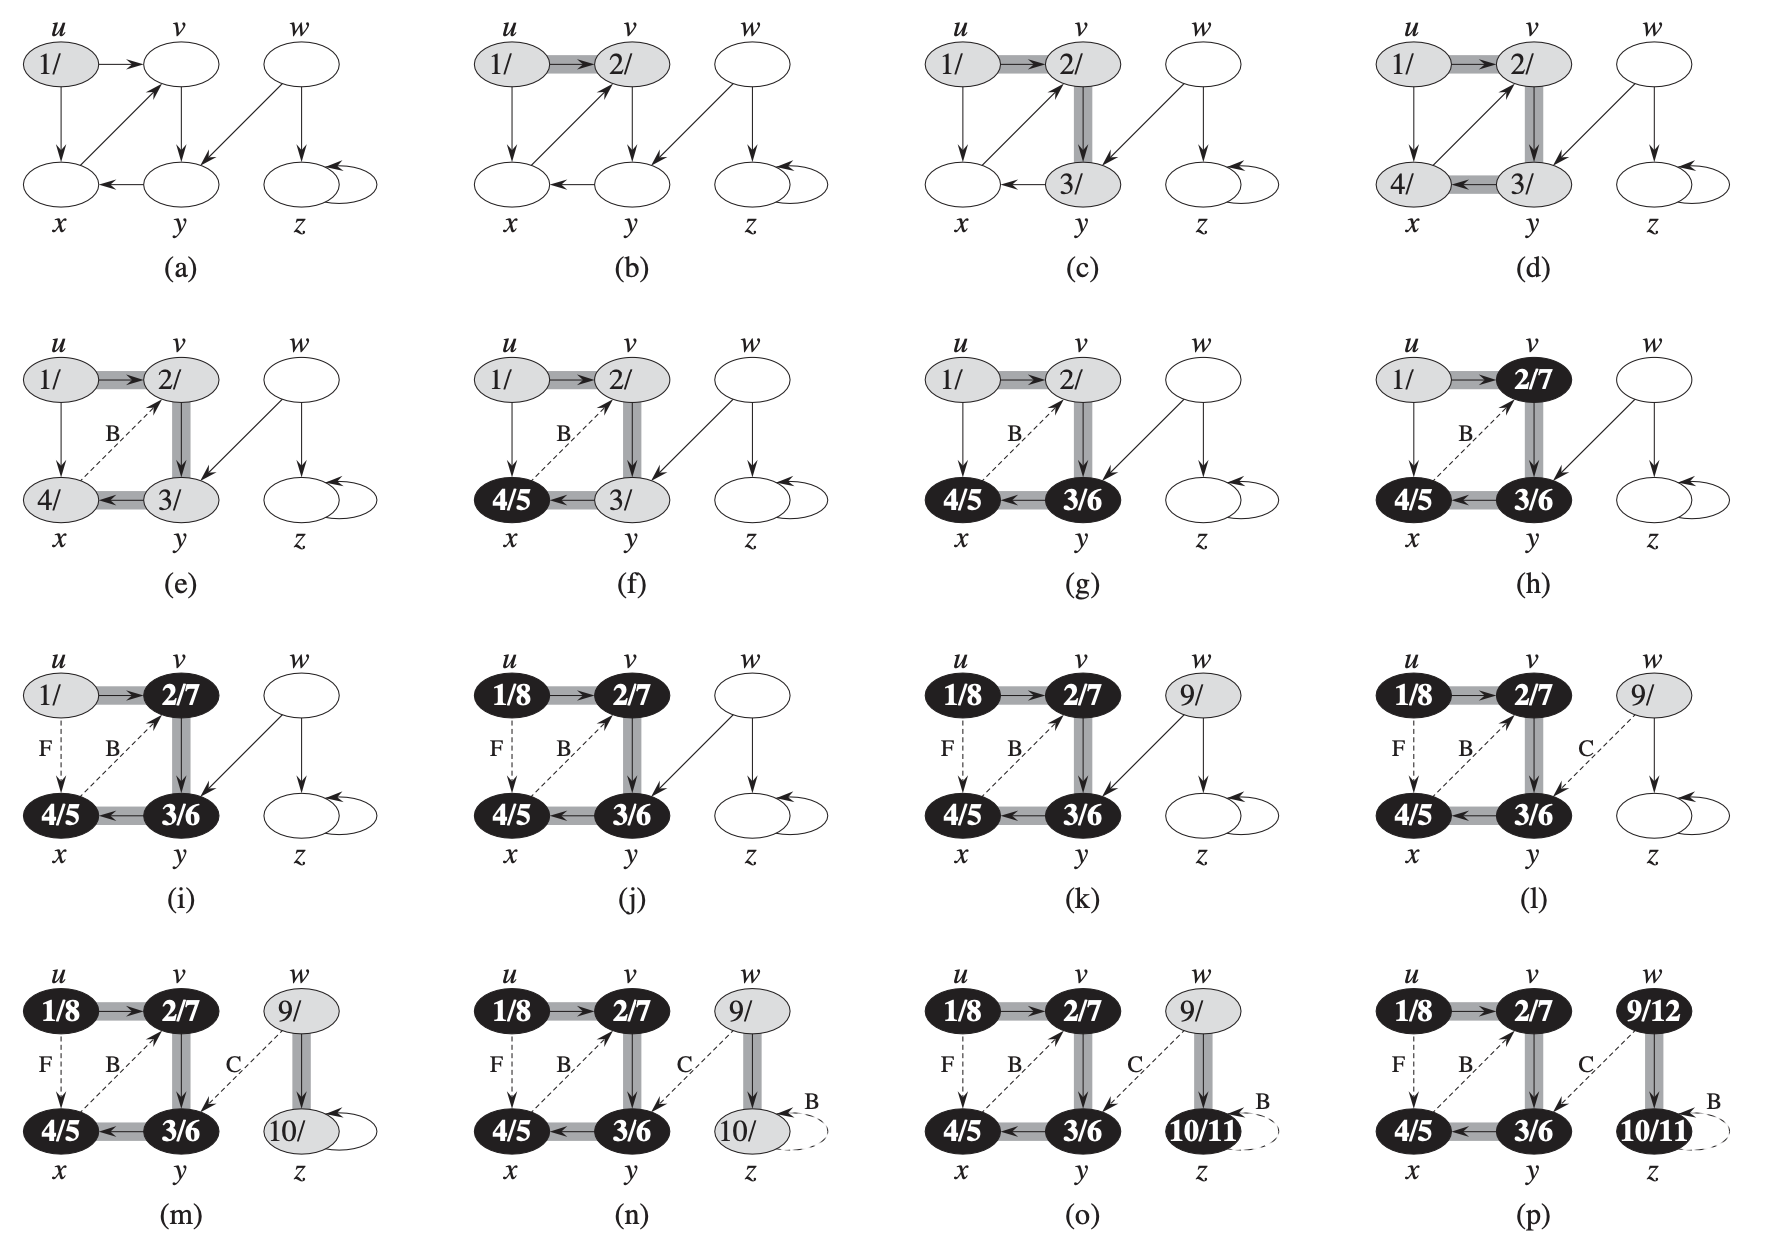
\includegraphics[width=\textwidth]{assets/dfs.png}
    \caption{Depth-First Search}
    \label{fig:dfs}
\end{figure}

\subsection*{Analysis}

The running time of depth-first search is $O(V + E)$, which is the same as the running time of breadth-first search. The time is proportional to the sum of the lengths of the adjacency lists of all the vertices. The depth-first search algorithm is a simple algorithm that is easy to implement and efficient when the graph is represented by the adjacency-list structure.
The running time of DFS consists of two main parts:
\begin{itemize}
    \item The loops on lines 1-3 and lines 5-7 of DFS take time $\Theta(V)$, where $V$ is the number of vertices in the graph.
    \item The time for executing the \texttt{DFS-VISIT} procedure.
\end{itemize}

Using aggregate analysis:
\begin{itemize}
    \item The procedure \texttt{DFS-VISIT} is called exactly once for each vertex $v \in V$, since a vertex is painted gray the first time it is visited.
    \item During an execution of \texttt{DFS-VISIT}$(G, v)$, the loop on lines 4-7 is executed $|Adj[v]|$ times, where $Adj[v]$ is the adjacency list of vertex $v$.
\end{itemize}

The total cost of all executions of lines 4-7 is:

$$
\sum_{v \in V} |Adj[v]| = \Theta(E),
$$

where $E$ is the number of edges in the graph.

Thus, the overall running time of DFS is:

$$
\Theta(V + E).
$$

\section{Topological Sort}

A \textbf{topological sort} of a directed acyclic graph $G = (V, E)$ is a linear ordering of all its vertices such that if $G$ contains an edge $(u, v)$, then $u$ appears before $v$ in the ordering. A topological sort of a directed acyclic graph is not unique. If the graph has a cycle, then no linear ordering is possible.

\begin{algorithm}[H]
    \caption{TOPOLOGICAL-SORT(G)}
    call DFS(G) to compute finishing times $v.f$ for each vertex $v$ \\
    as each vertex is finished, insert it onto the front of a linked list \\
    return the linked list of vertices
\end{algorithm}

We can perform a topological sort in time $O(V + E)$, since the time to call DFS is $O(V + E)$ and the time to insert each of the $V$ vertices onto the front of the linked list is $O(1)$.

\section{Dijkstra's Algorithm}

Dijkstra's algorithm solves the single-source shortest-paths problem on a weighted, directed graph $G = (V, E)$ for the case in which all edge weights are nonnegative.
It maintains a set $S$ of vertices whose final shortest-path
weights from the source $s$ have already been determined. The algorithm repeatedly selects the vertex $u \in V - S$
with the minimum shortest-path estimate, adds $u$ to $S$, and relaxes all edges leaving $u$.

Because it always chooses the "lightest" or "closest" vertex in $V - S$ to add to set $S$, we say that it uses a greedy strategy.

\begin{theorem}
    Dijkstra’s algorithm, run on a weighted, directed graph $G = (V, E)$ with non-negative weight function w and source s, terminates with $u.d = \delta(s, u) \forall u \in V$.
\end{theorem}
\begin{proof}
    We prove this theorem by induction on the number of vertices in the set $S$.

    \textbf{Base case:} Initially, $S = \emptyset$ and $s.d = 0 = \delta(s, s)$. For all other vertices $v \in V \setminus \{s\}$, $v.d = \infty \geq \delta(s, v)$. Thus, the base case holds.

    \textbf{Inductive step:} Assume that for any vertex $u \in S$, $u.d = \delta(s, u)$. We need to show that when a vertex $v$ is added to $S$, $v.d = \delta(s, v)$.

    Let $v$ be the next vertex added to $S$. By the inductive hypothesis, for all vertices $u \in S$, $u.d = \delta(s, u)$. Since $v$ is chosen as the vertex with the minimum shortest-path estimate, $v.d \leq u.d + w(u, v)$ for all edges $(u, v) \in E$ where $u \in S$.

    Consider any path $p$ from $s$ to $v$. Let $u$ be the last vertex on the path $p$ that is in $S$. Then, the subpath from $s$ to $u$ is a shortest path, and $u.d = \delta(s, u)$. The weight of the subpath from $u$ to $v$ is at least $w(u, v)$. Therefore, the total weight of the path $p$ is at least $\delta(s, u) + w(u, v) = u.d + w(u, v) \geq v.d$. Thus, $v.d \leq \delta(s, v)$.

    Since $v.d$ is a shortest-path estimate and cannot be less than the actual shortest-path distance, $v.d \geq \delta(s, v)$. Combining these inequalities, we get $v.d = \delta(s, v)$.

    Thus, by induction, for each vertex $u \in V$, the value $u.d$ computed by Dijkstra's algorithm satisfies $u.d = \delta(s, u)$.
\end{proof}

\begin{figure}[H]
    \centering
    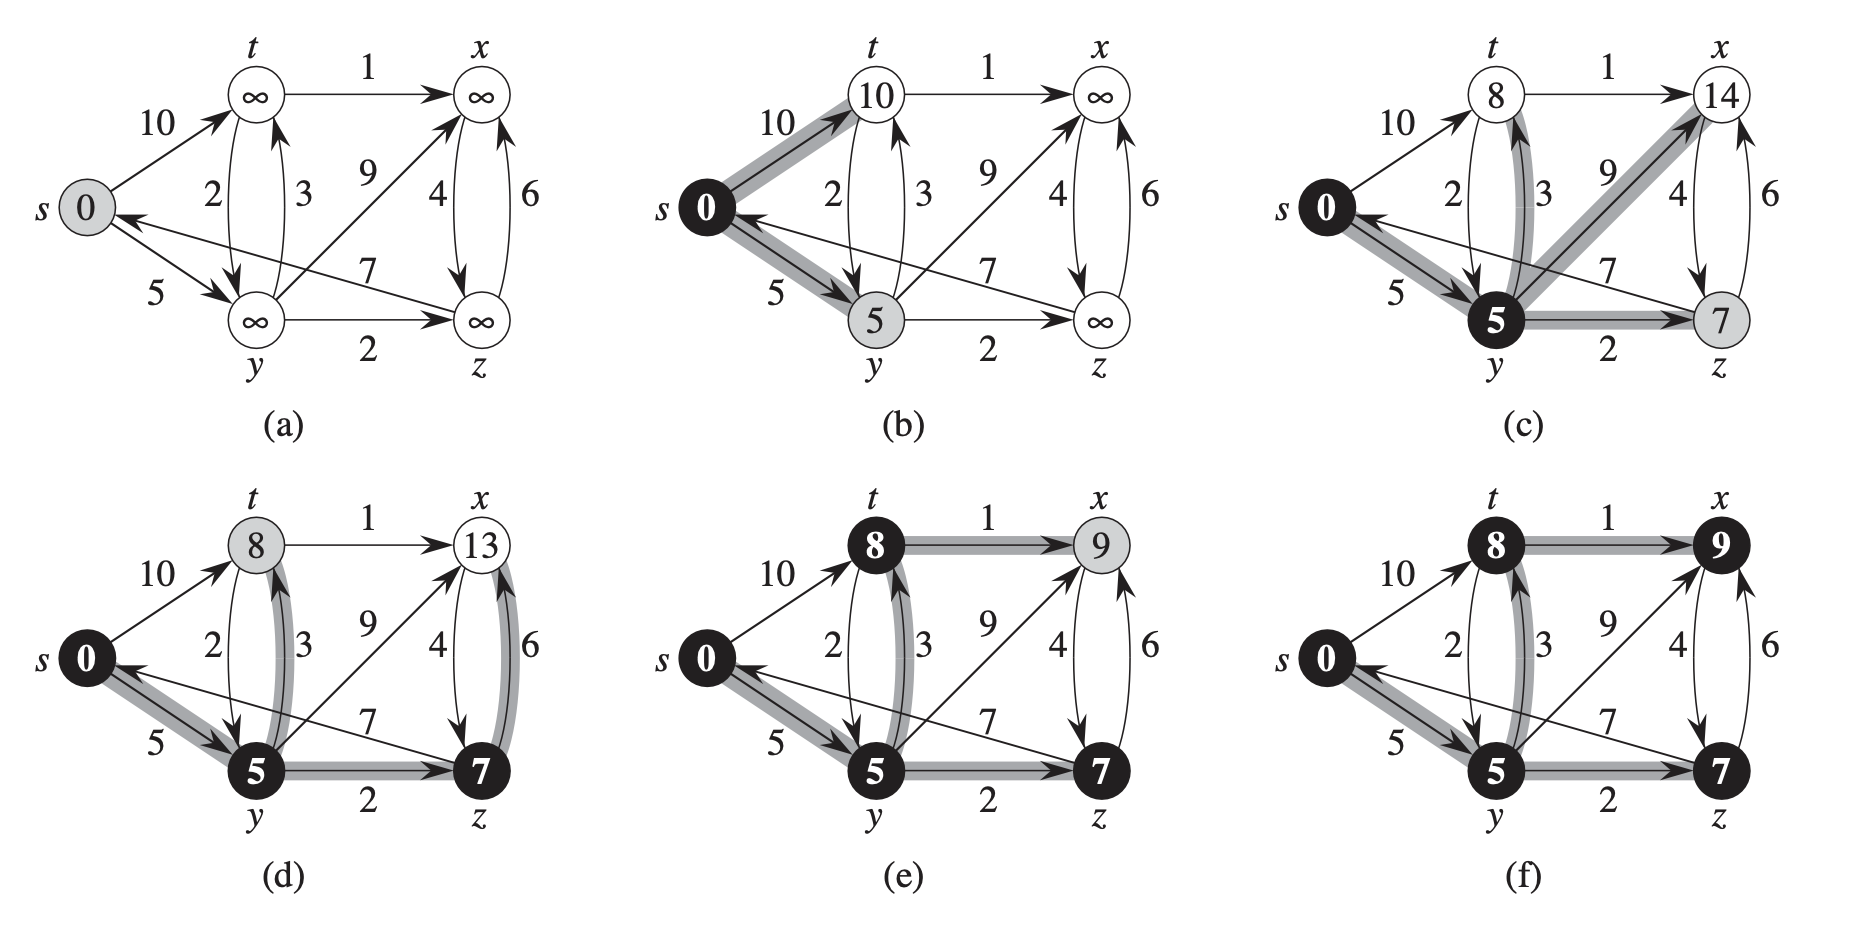
\includegraphics[width=0.9\textwidth]{assets/dijkstra.png}
    \caption{Dijkstra's Algorithm}
    \label{fig:dijkstra}
\end{figure}

\subsection*{Analysis}
The running time of Dijkstra's algorithm depends on how the priority queue is implemented. Let's analyze the running time for different implementations of the priority queue.

\begin{itemize}
    \item \textbf{Using a binary min-heap:} 
    \begin{itemize}
        \item The initialization of the single source takes $O(V)$ time.
        \item The priority queue operations (insert, extract-min, and decrease-key) take $O(\log V)$ time each.
        \item The algorithm performs $|V|$ extract-min operations, each taking $O(\log V)$ time, for a total of $O(V \log V)$.
        \item The algorithm performs $|E|$ decrease-key operations, each taking $O(\log V)$ time, for a total of $O(E \log V)$.
    \end{itemize}
    Therefore, the total running time using a binary min-heap is $O((V + E) \log V)$.

    \item \textbf{Using a Fibonacci heap:}
    \begin{itemize}
        \item The initialization of the single source takes $O(V)$ time.
        \item The insert and decrease-key operations take $O(1)$ amortized time each.
        \item The extract-min operation takes $O(\log V)$ amortized time.
        \item The algorithm performs $|V|$ extract-min operations, each taking $O(\log V)$ amortized time, for a total of $O(V \log V)$.
        \item The algorithm performs $|E|$ decrease-key operations, each taking $O(1)$ amortized time, for a total of $O(E)$.
    \end{itemize}
    Therefore, the total running time using a Fibonacci heap is $O(V \log V + E)$.
\end{itemize}

In summary, the running time of Dijkstra's algorithm is $O((V + E) \log V)$ when using a binary min-heap and $O(V \log V + E)$ when using a Fibonacci heap. The latter is more efficient for dense graphs where $|E|$ is large.